\documentclass{beamer}
\usepackage[utf8x]{inputenc}
\usepackage{color}
\usepackage{listings}
\usepackage{graphicx} % needed for beamer

\lstset{%
  language=sh, % FIXME: nice syntax coloring for JSON
  basicstyle=\ttfamily\footnotesize,
	showspaces=false,
	showstringspaces=false,
	showtabs=false,
	keepspaces=true,
	%breaklines=true,
}

\usetheme{Boadilla}
\usefonttheme{professionalfonts}
\useoutertheme[subsection=false,footline=empty]{miniframes}
\useinnertheme{circles}
\setbeamertemplate{footline}[frame number]

\author{slopjong, rohieb}
\title{SpaceAPI}
\subtitle{Dezentrales Hackerspace-Informationssystem}
\institute{GPN13}
\date{1. Juni 2013}

\begin{document}
\begin{frame}
	\maketitle
\end{frame}

\section{Motivation}
\begin{frame}{Motivation}
	Jeder Hackerspace kennt das Problem\ldots
	\begin{center}
	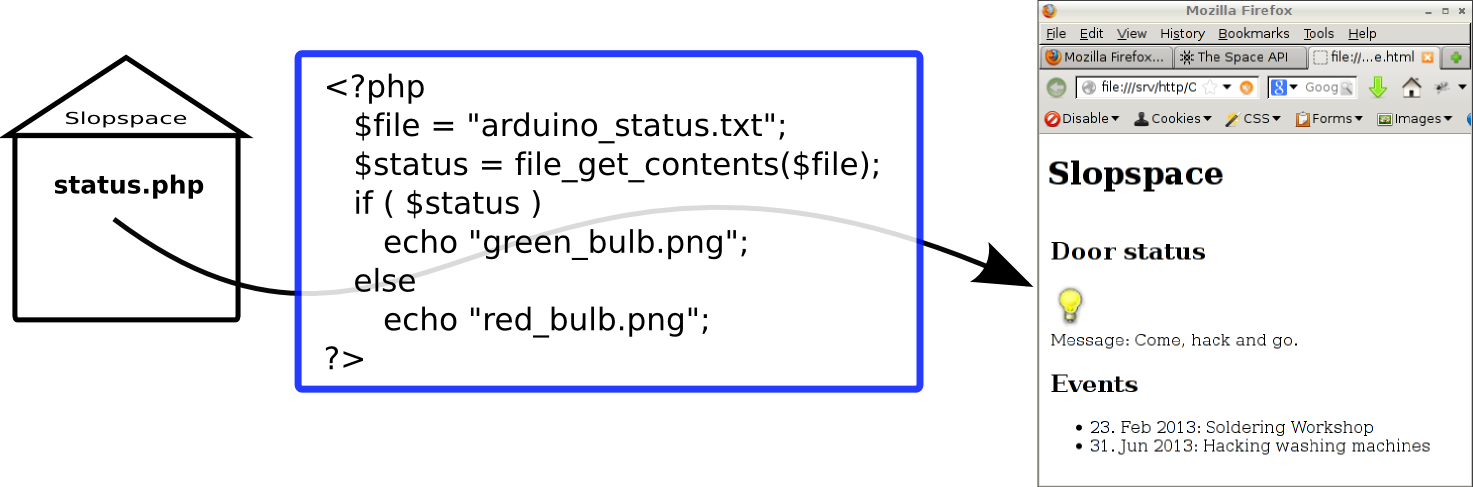
\includegraphics[width=0.9\textwidth]{openclose-impl.png}
	\end{center}
\end{frame}

\begin{frame}{Motivation}
\begin{itemize}
	\item einheitliche API für Metadaten über Hackerspaces
	\pause
	\begin{itemize}
		\item Adressen
		\item Kontaktdaten
		\item Events
		\item \ldots you name it.
	\end{itemize}
	\pause
	\item because we can
	\item more dataporn
\end{itemize}
\end{frame}

\section{Architektur}
\begin{frame}{Architektur}
\begin{itemize}
	\item HTTP
	\item JSON
	\item dezentral!
	\begin{itemize}
		\item Endpoints
		\item OpenSpace Directory
	\end{itemize}
\end{itemize}
\end{frame}

\subsection{OpenSpace Directory}
\begin{frame}[fragile]{OpenSpace Directory}
\texttt{GET} \url{http://spaceapi.net/directory.json}
\begin{itemize}
	\item Mapping Hackerspace-Name $\Rightarrow$ Endpoint-URL
	\item Attribut-Filter
\end{itemize}

\begin{lstlisting}
$ curl http://spaceapi.net/directory.json?filter=cam
{
  "Ace Monster Toys":"http:\/\/acemonstertoys.org\/status.json",
  "Bitlair":"https:\/\/bitlair.nl\/statejson.php",
  "FamiLAB":"http:\/\/familab.org\/status\/status.php",
  "Farset Labs":"http:\/\/openspace.slopjong.de\/cache\/Farset+Labs",
  [...]
}
\end{lstlisting}
\end{frame}

\begin{frame}{ALL the Spaces}
	\begin{center}
		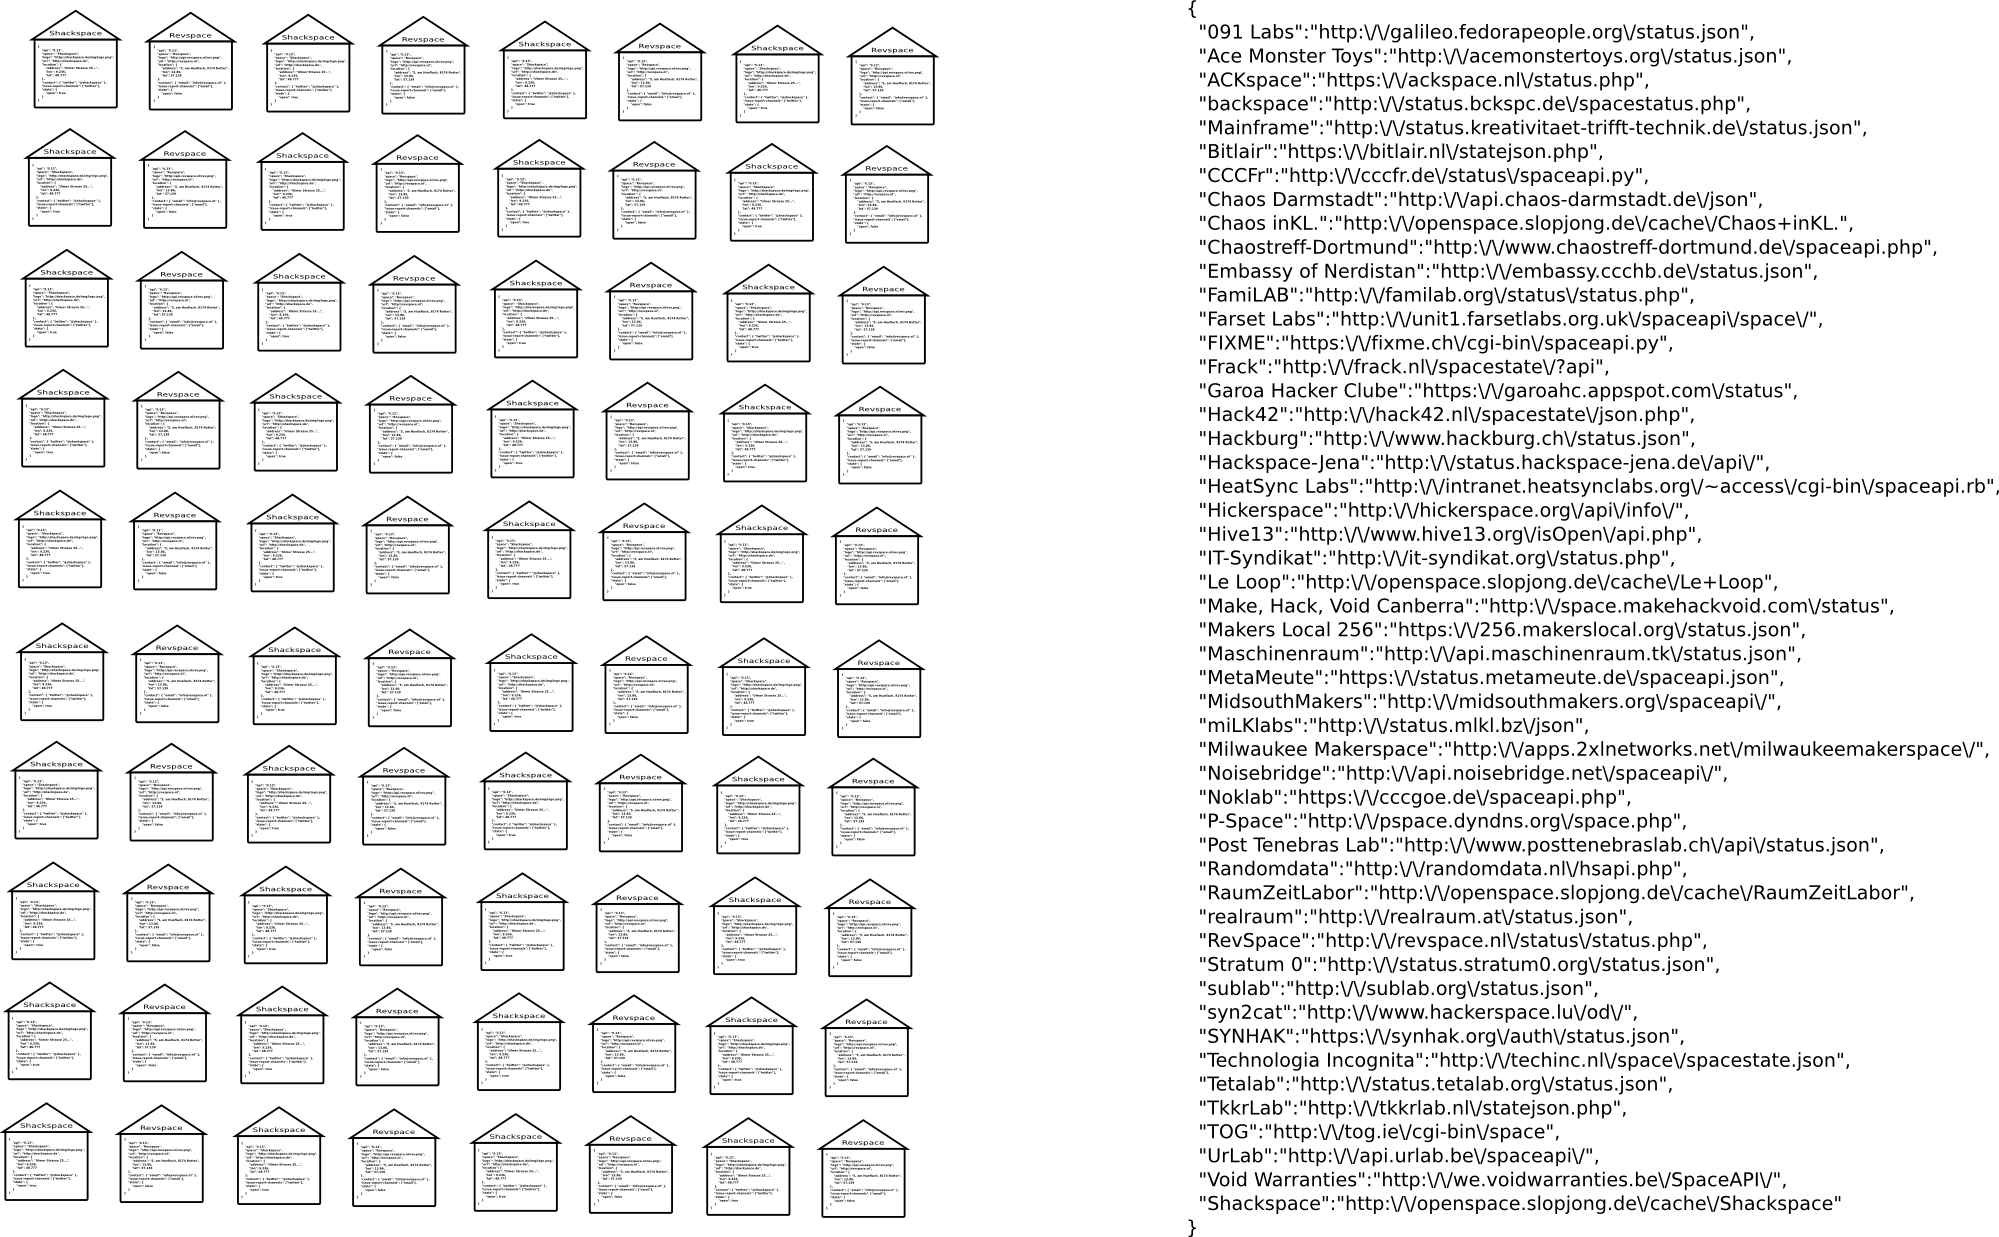
\includegraphics[width=0.9\textwidth]{allthespaces.png}
	\end{center}
\end{frame}

\subsection{Endpoints}
\begin{frame}[fragile]{Endpoints}
\begin{lstlisting}
$ curl http://status.stratum0.org/status.json
{
  "api": "0.12",
  "space": "Stratum 0",
  "url": "https:\/\/stratum0.org",
  "logo": "https:\/\/stratum0.org\/mediawiki\/images\/thumb\/c\/c6\/Sanduhr-twitter-avatar-black.svg\/240px-Sanduhr-twitter-avatar-black.svg.png",
  "address": "Hamburger Strasse 273a, 38114 Braunschweig, Germany",
  "lon": 10.5211247, "lat": 52.2785658,
  "lastchange": 1369899560
  "open": true, "status": "We're open for public",
  "contact": {
    "phone": "+4953128769245",
    "twitter": "@stratum0",
    "ml": "normalverteiler@stratum0.org",
    "irc": "irc:\/\/irc.freenode.net\/#stratum0" },
  "icon": {
    "open": "http:\/\/status.stratum0.org\/open_square.png",
    "closed": "http:\/\/status.stratum0.org\/closed_square.png"
  } }
\end{lstlisting}
\end{frame}

\section{Apps}
\begin{frame}{Hackerspace Globe}
\begin{center}
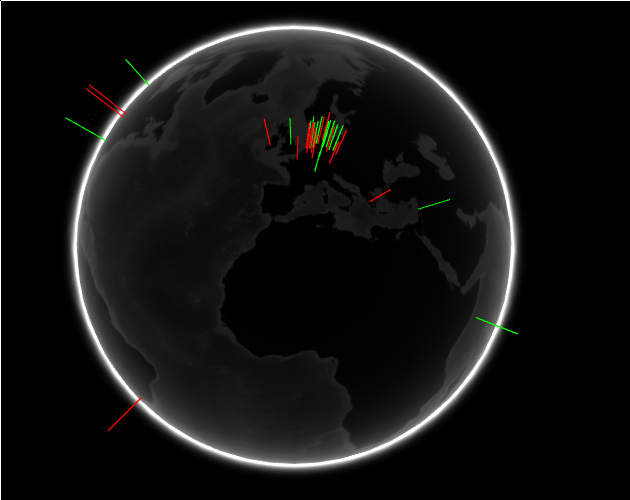
\includegraphics[height=0.7\textheight]{hackerspace-globe.png}

\url{http://joewalnes.github.io/hackerspace-globe/}
\end{center}
\end{frame}

\begin{frame}{Hackerspace Globe}
\begin{center}
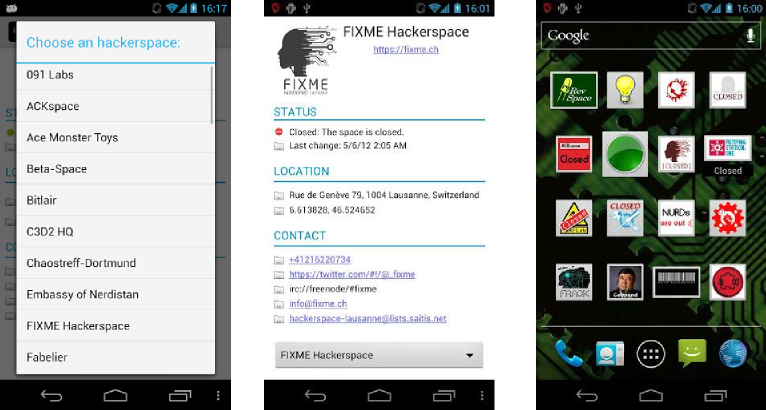
\includegraphics[height=0.7\textheight]{my-hackerspace.png}

\url{https://github.com/fixme-lausanne/MyHackerspace}
\end{center}
\end{frame}

\begin{frame}[fragile]{Kontakt}
\begin{itemize}
	\item \url{http://spaceapi.net}
	\item Mailingliste:
		\url{http://lists.hackerspaces.org/mailman/listinfo/spaceapi-devel}
	\item IRC: \texttt{\#spaceapi} auf FreeNode
\end{itemize}
\end{frame}
\end{document}
